\documentclass[../document.tex]{subfiles}
\begin{document}\label{ssec:time}

\begin{figure*}
\begin{minipage}[b]{.45\textwidth}
\centering
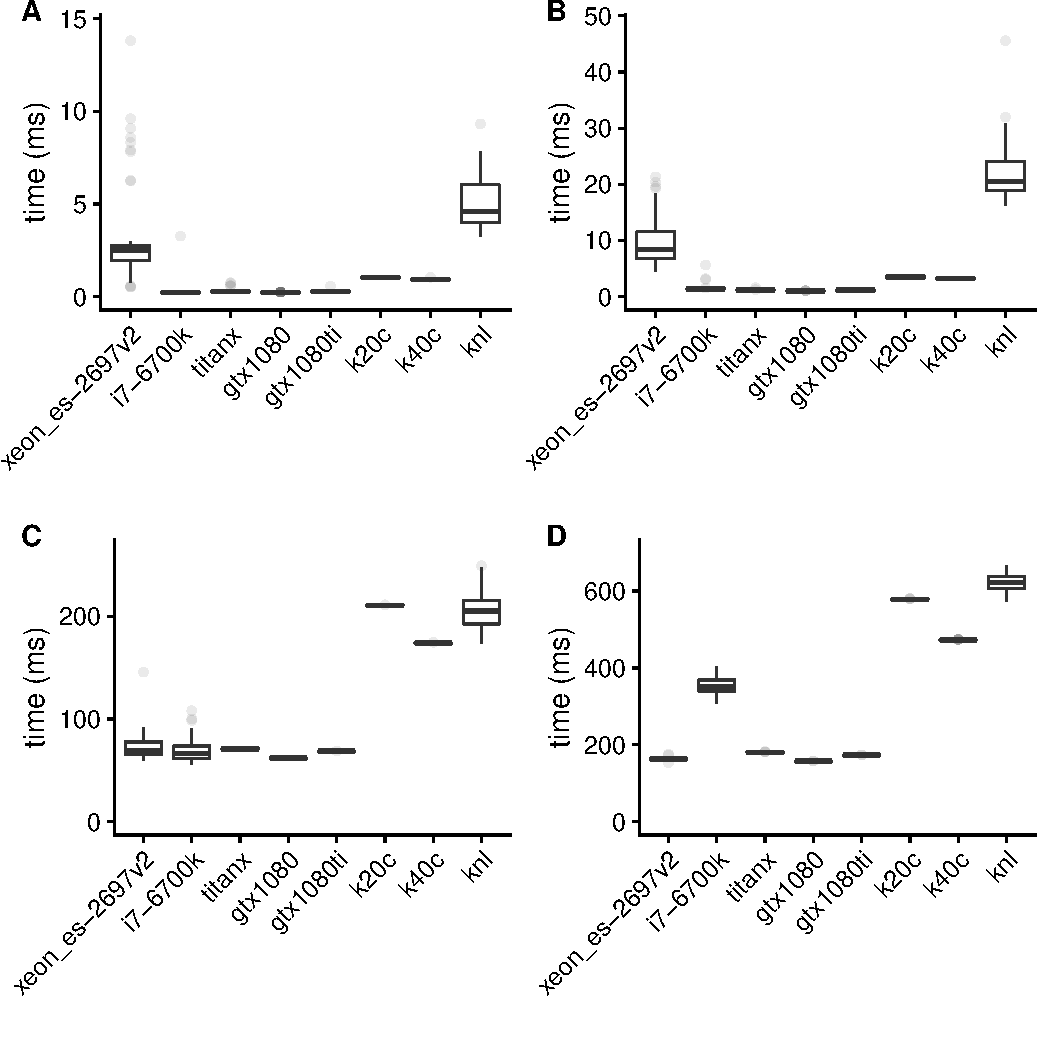
\includegraphics[width=1\textwidth]{figures/time-results/kmeans.pdf}
\caption{Kernel Execution times of the {\bf lud} benchmark.}
\label{fig:time-kmeans}
\end{minipage}
\hfill
\begin{minipage}[b]{.45\textwidth}
\centering
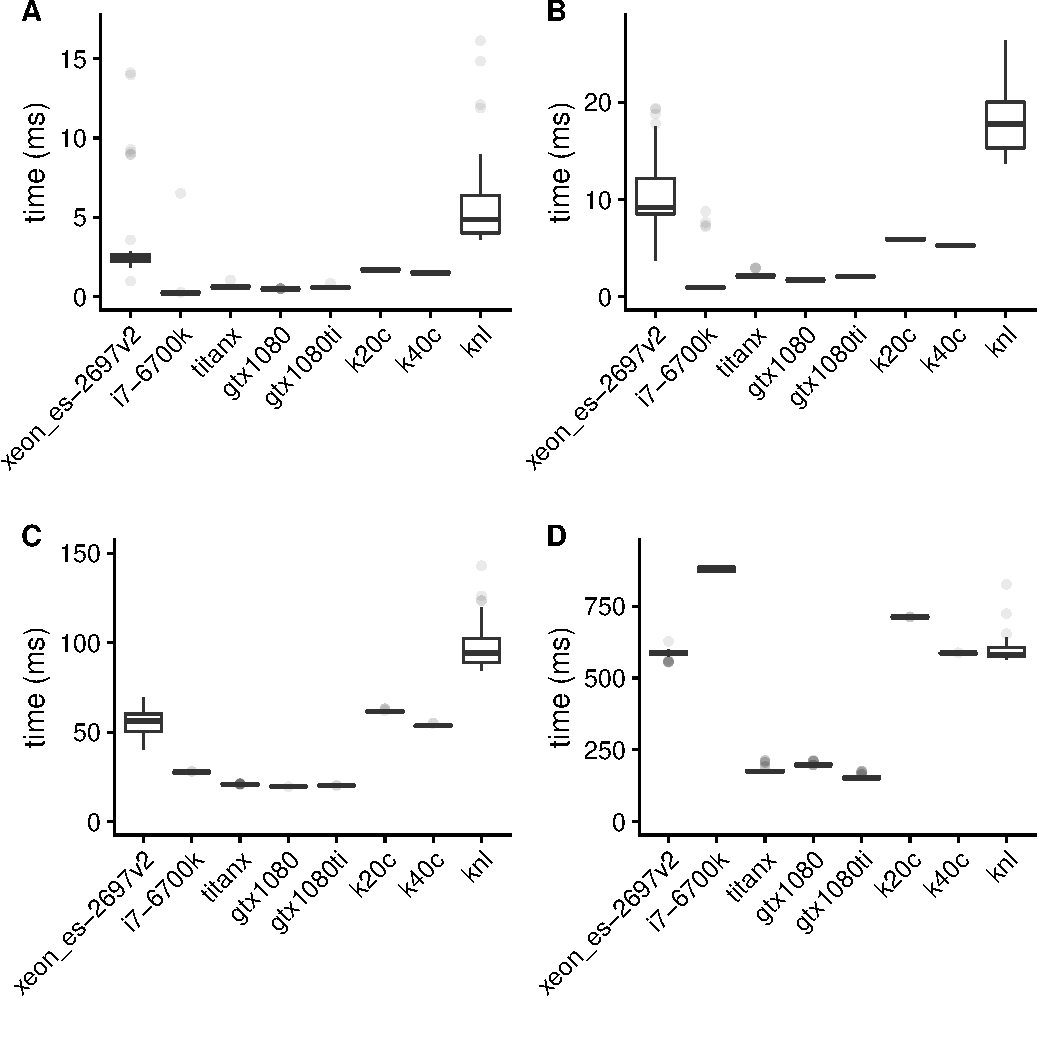
\includegraphics[width=1\textwidth]{figures/time-results/lud.pdf}
\caption{Kernel execution times over the {\bf lud} benchmark.}
\label{fig:time-lud}
\end{minipage}
\end{figure*}

\begin{figure*}
\begin{minipage}[b]{.45\textwidth}
\centering
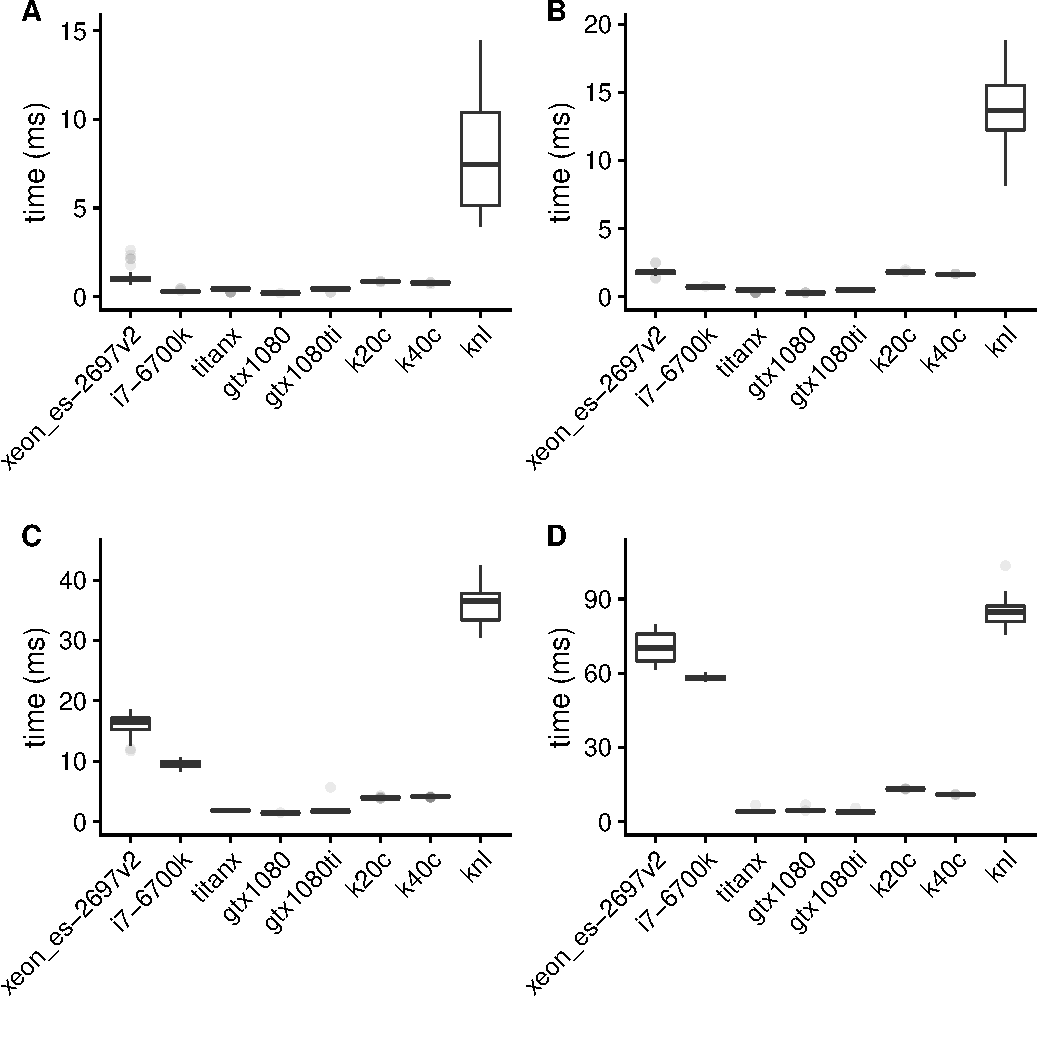
\includegraphics[width=1\textwidth]{figures/time-results/dwt.pdf}
\caption{Kernel Execution times for {\bf dwt}.}
\label{fig:time-dwt}
\end{minipage}
\hfill
\begin{minipage}[b]{.45\textwidth}
\centering
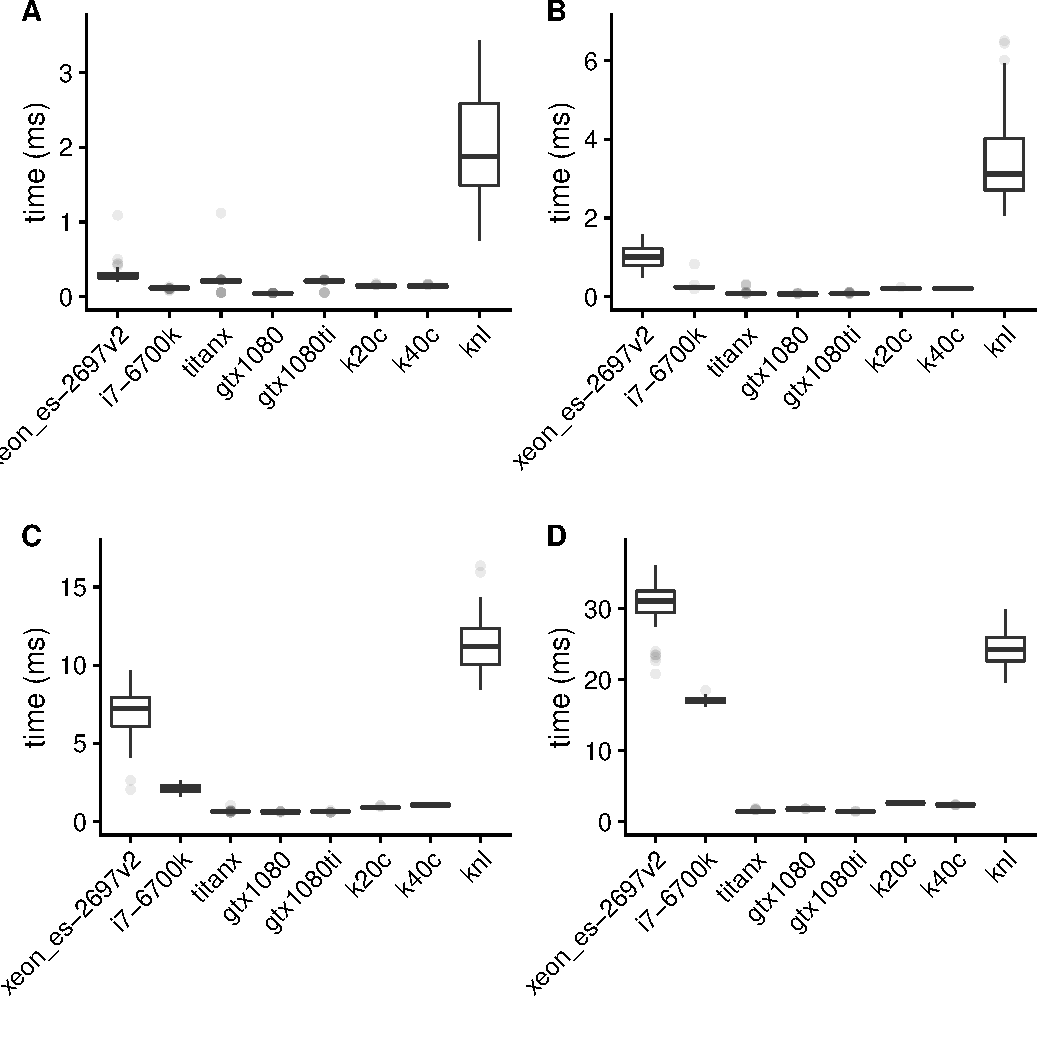
\includegraphics[width=1\textwidth]{figures/time-results/fft.pdf}
\caption{Kernel execution times for {\bf fft}.}
\label{fig:time-fft}
\end{minipage}
\end{figure*}

\begin{figure*}
\begin{minipage}[b]{.45\textwidth}
\centering
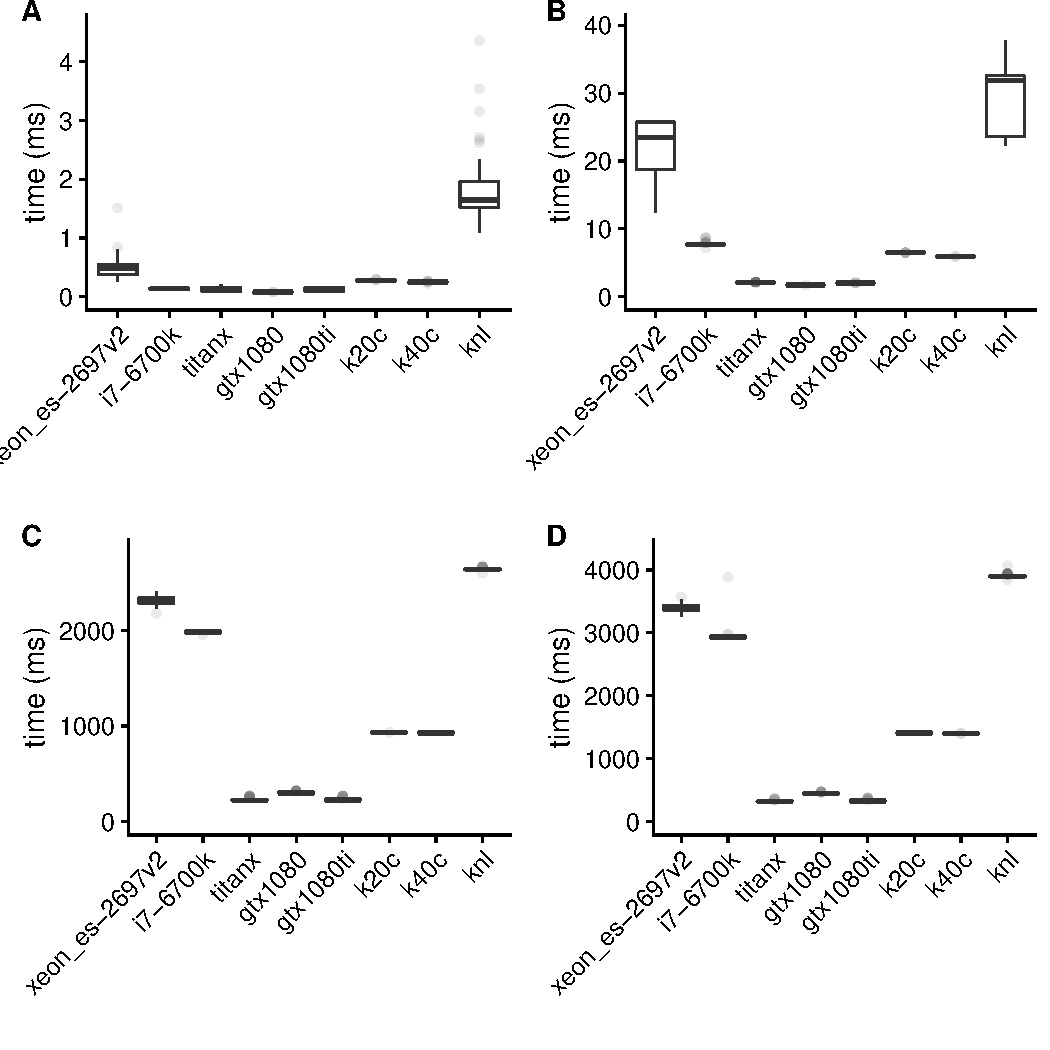
\includegraphics[width=1\textwidth]{figures/time-results/gem.pdf}
\caption{Kernel Execution times for {\bf gem}.}
\label{fig:time-gem}
\end{minipage}
\hfill
\begin{minipage}[b]{.45\textwidth}
\centering
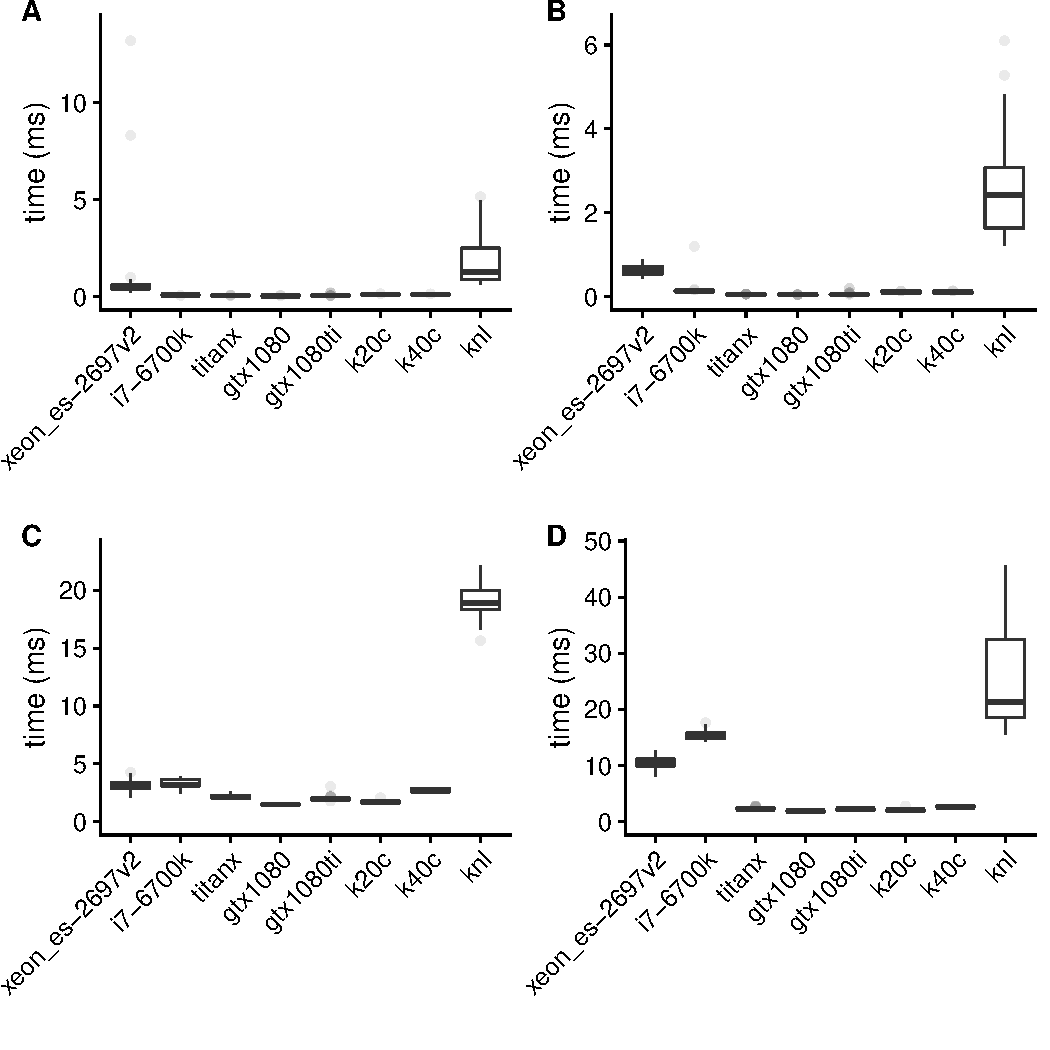
\includegraphics[width=1\textwidth]{figures/time-results/srad.pdf}
\caption{Kernel execution times for {\bf srad}.}
\label{fig:time-srad}
\end{minipage}
\end{figure*}

\begin{figure*}
\centering
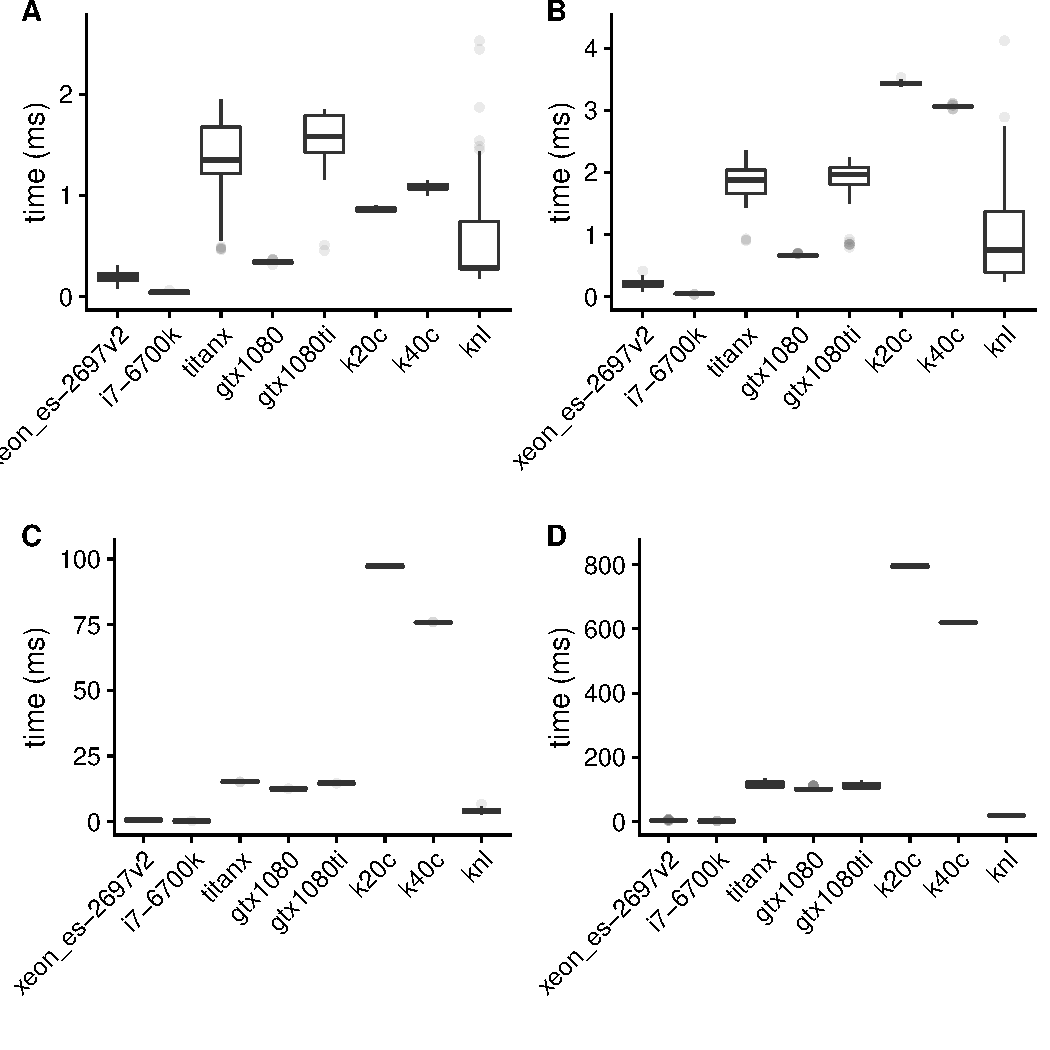
\includegraphics[width=1\textwidth]{figures/time-results/crc.pdf}
\caption{Kernel Execution times for {\bf crc}.}
\label{fig:time-crc}
\end{figure*}

Sample execution times from running 50 iterations per benchmark application.
The top-left corner captions in all figures correspond to the 4 different workload sizes, such that {\bf A} corresponds to {\bf tiny}, {\bf B} corresponds to {\bf small}, {\bf C} to {\bf medium} and {\bf D} to {\bf large}.

The first two sets of figures in a row have applications which both correspond to a particular dwarf, for instance Figure~\ref{fig:time-kmeans} and Figure~\ref{fig:time-lud} are both representative of the Dense Linear Algebra dwarf, whereas Figure~\ref{fig:time-dwt} and Figure~\ref{fig:time-fft} are both applications within Spectral Methods.

Figure~\ref{fig:time-gem} represents N-Body Methods, Figure~\ref{fig:time-srad} encompasses a Structured Grid Method of Dwarf, and finally Figure~\ref{fig:time-crc} is a problem from Combinational Logic.

\end{document}
